% VLDB template version of 2020-08-03 enhances the ACM template, version 1.7.0:
% https://www.acm.org/publications/proceedings-template
% The ACM Latex guide provides further information about the ACM template

\documentclass[sigconf, nonacm]{acmart}
\usepackage{mathtools}
\usepackage{amsfonts}
\usepackage{caption}
\usepackage{subfig}
\usepackage{changepage}
\usepackage{amsthm}

%% The following content must be adapted for the final version
% paper-specific
\newcommand\vldbdoi{XX.XX/XXX.XX}
\newcommand\vldbpages{XXX-XXX}
% issue-specific
\newcommand\vldbvolume{14}
\newcommand\vldbissue{1}
\newcommand\vldbyear{2020}
% should be fine as it is
\newcommand\vldbauthors{\authors}
\newcommand\vldbtitle{\shorttitle} 
% leave empty if no availability url should be set
\newcommand\vldbavailabilityurl{URL_TO_YOUR_ARTIFACTS}
% whether page numbers should be shown or not, use 'plain' for review versions, 'empty' for camera ready
\newcommand\vldbpagestyle{plain} 

\begin{document}
\title{A Thorough Analysis of and Improvement on UMAP and tSNE}

%%
%% The "author" command and its associated commands are used to define the authors and their affiliations.
\author{Andrew}
\author{Jakob}
\author{Katrine}
\affiliation{%
  \institution{Aarhus University}
  \streetaddress{}
  \city{}
  \state{}
  \postcode{}
}
\email{draganovandrew@cs.au.dk}
%%
%% The abstract is a short summary of the work to be presented in the
%% article.
\begin{abstract}
Dimensionality reduction algorithms are used across scientific disciplines to visualize and understand data. Among them, tSNE and UMAP have become two of the most
popular due to their quick runtimes and intuitive results. However, despite their ubiquity and similarities there
has not been a comprehensive comparison of the two approaches. In this work, we describe a general framework for comparing dimensionality reduction algorithms and
identify simple methods for obtaining each algorithm from the other. We disprove several claims regarding the source of the algorithms' efficacy and clarify
misconceptions regarding components of each algorithm. Inspired by this, we create a new dimensionality reduction algorithm, Uniform UMAP, by combining the best characteristics of tSNE
and UMAP. Uniform UMAP can recreate the results of both tSNE \& UMAP and, when executed in a single thread, performs the optimizations an order of magnitude faster than
multi-threaded UMAP and several orders of magnitude faster than multi-threaded tSNE on even modestly sized datasets. We additionally highlight that Uniform UMAP is easier to parallelize than either of the previous approaches and provide
a simple GPU implementation for yet another order of magnitude speedup.
Lastly, we provide theoretical insights for future dimensionality reduction improvements.
\end{abstract}

\maketitle

%%% do not modify the following VLDB block %%
%%% VLDB block start %%%
\pagestyle{\vldbpagestyle}
\begingroup\small\noindent\raggedright\textbf{PVLDB Reference Format:}\\
\vldbauthors. \vldbtitle. PVLDB, \vldbvolume(\vldbissue): \vldbpages, \vldbyear.\\
\href{https://doi.org/\vldbdoi}{doi:\vldbdoi}
\endgroup
\begingroup
\renewcommand\thefootnote{}\footnote{\noindent
This work is licensed under the Creative Commons BY-NC-ND 4.0 International License. Visit \url{https://creativecommons.org/licenses/by-nc-nd/4.0/} to view a copy of this license. For any use beyond those covered by this license, obtain permission by emailing \href{mailto:info@vldb.org}{info@vldb.org}. Copyright is held by the owner/author(s). Publication rights licensed to the VLDB Endowment. \\
\raggedright Proceedings of the VLDB Endowment, Vol. \vldbvolume, No. \vldbissue\ %
ISSN 2150-8097. \\
\href{https://doi.org/\vldbdoi}{doi:\vldbdoi} \\
}\addtocounter{footnote}{-1}\endgroup
%%% VLDB block end %%%

%%% do not modify the following VLDB block %%
%%% VLDB block start %%%
\ifdefempty{\vldbavailabilityurl}{}{
\vspace{.3cm}
\begingroup\small\noindent\raggedright\textbf{PVLDB Artifact Availability:}\\
The source code, data, and/or other artifacts have been made available at \url{\vldbavailabilityurl}.
\endgroup
}
%%% VLDB block end %%%

\section{Introduction}
Dimensionality reduction (DR) algorithms are invaluable for qualitatively inspecting high-dimensional data. As such, they are consistently used across the sciences
with famous applications in \_\_\_\_, \_\_\_\_, and \_\_\_\_. A DR algorithm receives an input dataset $X \in \mathbb{R}^{N \times D}$ of
$N$ points in $D$ dimensional space and
attempts to find a faithful embedding into a lower dimensional space $Y \in \mathbb{R}^{N \times d}$, where $d << D$. The term \textit{faithful} is
defined as keeping similar points similar and dissimilar points dissimilar, where similarity is commonly measured by distance metrics or kernels in the
corresponding spaces. In this paper, we refer to the pairwise squared distance matrices in high- and low-dimensional spaces as $E^X$ and $E^Y$, respectively.

Recent approaches model the problem in terms of the minimization of some objective function $\mathcal{L}(f(E^X), g(E^Y))$, where $f$ and $g$ are high- and
low-dimensional functions with respect to the distances. They then employ gradient descent to overcome the lack of clear closed-form solutions. We
focus on the tSNE \cite{van2008visualizing} and UMAP \cite{mcinnes2018umap} gradient descent-based algorithms, which have become standard DR
techniques in recent years --- each getting cited more than
1000 times per year on average. Despite both their ubiquity and similarity, though, there has not been a thorough analysis of the different design choices
     between the two methods.

In this paper, we first identify every framework choice and implementation discrepancy that differs between tSNE and UMAP. This allows us to describe each algorithm as a set of on/off
switches across the space of these differences. We then implement tSNE and UMAP in a common library, giving us the ability to study the effect of each
design choice on each of the algorithms.
We provide evidence that the most relevant changes are the choice of normalization on $E^X$ and $E^Y$ and the choice of gradient descent algorithm by showing that the other design choices do not have a consistent or significant effect on the resulting embeddings.

Based on this analysis we propose Uniform UMAP, a method that can recreate both tSNE and UMAP results by changing just two input parameters. Additionally, our
method obtains a significant speedup on UMAP and a multiple-order-of-magnitude speedup on tSNE by choosing the more efficient options among the
irrelevant design choices.
Furthermore, our library includes GPU code and simpler objective functions for further speedups, providing the fastest implementation for achieving the results
from both tSNE and UMAP in
a fully plug-and-play manner with respect each algorithm's current popular implementation.


% \section{Comparison of tSNE and UMAP} \label{comparison}
% We begin by formally introducing the tSNE and UMAP DR algorithms. Let $X \in \mathbb{R}^{N \times D}$ be the high dimensional dataset of $N$ points and let $Y
% \in \mathbb{R}^{N \times d}$ be a previously initialized set of $N$ points in lower-dimensional space such that $d << D$. 
% 
% We now respectively establish Gaussian and student-t kernels on the high- and low-dimensional distances to represent the likelihood that $x_i$ and $y_i$ choose
% $x_j$ and $y_j$ as their respective nearest neighbors. These kernels are defined by
% \begin{align}
%     % FIXME - the denominator here isn't quite right
%     p^{tsne}_{j|i}(x_i, x_j) &= \dfrac{\text{exp}(-d(x_i, x_j)^2 / 2 \sigma_i^2)}{\sum_{k \neq l} \text{exp}(-d(x_k, x_l)^2 / 2 \sigma_k^2)} \\[0.5ex]
%     q^{tsne}_{ij}(y_i, y_j) &= \dfrac{(1 + ||y_i - y_j||^2_2)^{-1}}{\sum_{k \neq l} (1 + ||y_k - y_l||^2_2)^{-1}} \\[1.5ex]
%     p^{umap}_{j|i}(x_i, x_j) &= \dfrac{\text{exp} (-d(x_i, x_j)^2 + \rho_{i})}{\tau_i} \\[0.3ex]
%     q^{umap}_{ij}(y_i, y_j) &= \left( 1 + a(||y_i - y_j||^2_2)^b \right) ^{-1}
% \end{align}
% where $d(x_i, x_j)$ is the high-dimensional distance function, $\sigma$ and $\tau$ are point-specific variance scalars, $\rho_i = \min_{j \neq i} d(x_i, x_j)$,
% and $a$ and $b$ are constants. In practice, we can assume that $2 \sigma_i^2$ is functionally equivalent to $\tau_i$, and we will use $\tau$ when referring to
% this kernel variance term. The high-dimensional kernels are symmetrized by applying symmetrization functions. Without loss of generality, let $p_{ij}
% = S(p_{j|i}, p_{i|j})$ for some symmetrization function $S$.
% 
% We posit that the primary difference between tSNE and UMAP is the change in normalization. tSNE normalizes the high- and low-dimensional kernels by all of the pairwise
% relations whereas UMAP allows the Gaussian and Student-t kernels to remain untouched\footnote{We note that the tSNE papers give the impression that
% high-dimensional normalization 
% occurs across rows, while in reality the code performs normalization across the entire pairwise kernel matrix.}. This implies a different probabilistic
% interpretation between the two algorithms. In the case of tSNE, the weights are normalized across the entire matrix of pairwise relations, giving us 
% a probability distribution across the entire dataset. In the case of UMAP, our pairwise kernels remain unnormalized, implying a Bernoulli distribution along
% each edge that can be interpreted as the likelihood of that edge existing (effectively independently from the other edges).
% 
% Each algorithm then applies gradient descent with respect to the KL-divergence(s) between these probability distributions. We refer to the high- and
% low-dimensional probability
% distributions as $P = \left( p_{ij} \right)_{i, j < N}$ and $Q = \left( q_{ij}
% \right)_{i, j < N}$ respectively. This gives us the loss functions
% \begin{align}
%     \mathcal{L}_{tsne} &= \text{KL} (P || Q) = \sum_{i \neq j} p_{ij} \log \dfrac{p_{ij}}{q_{ij}} \\
%     \mathcal{L}_{umap} &= \sum_{i \neq j} \left[ p_{ij} \log \dfrac{p_{ij}}{q_{ij}} + (1 - p_{ij}) \log \dfrac{1 - p_{ij}}{1 - q_{ij}} \right]
% \end{align}
% In essence, tSNE minimizes the KL divergence of the low- and high-dimensional pairwise distance matrices under their respective kernels, whereas UMAP sums over
% each edge's KL divergence in terms of the Bernoulli distribution.
% 
% \subsection{Intuition}
% 
% We would like to provide some intuition for these two normalizations. In the normalized case we have a probability distribution over all
% distinct pairwise relationships $p(x_i, x_j)$ and $q(y_i, y_j)$ for $i \neq j$. In the unnormalized case we instead have a probability distribution over each
% individual distinct pairwise relationship. We can look at these through the lens of a fully-connected graphs in which each edge $e_{ij}$ is the
% kernel value $p(x_i, x_j)$ or $q(y_i, y_j)$. Under this lens, the probabilities in the normalized case are akin to asking ``when we pick a random edge, what is the
% probability that we pick $e_{ij}$?''. Alternatively, the unnormalized variant asks ``for the specific edge $e_{ij}$, what is the probability that it exists?''
% Minimizing the KL divergence therefore amounts to ensuring that these probabilities in the high- and low-dimensional spaces are as similar as possible.
% 
% In practice, both tSNE and UMAP optimize this KL divergence by separately calculating attractive and repulsive forces. It is, however, unnecessary to calculate
% each such attraction and repulsion as, for example, dissimilar points in the high-dimensional space impose negligible attraction in the low-dimensional space.
% To simplify the complexity, both approaches establish a nearest neighbor graph \cite{van2014accelerating} with edges $|\mathcal{E}|$ among the
% high-dimensional points where points $x_i$ and $x_j$ share an edge if either $x_i$ is $x_j$'s nearest neighbor \underline{or} $x_j$ is $x_i$'s nearest neighbor.
% Then both algorithms simply perform attractions along these edges while performing repulsions evenly across the rest of the points. In this sense, we can
% interpret the gradient descent problem as a set of springs between every pair of points in $Y$ where the spring constants are determined by the Gaussian and
% Student-t kernels.
% 
% \subsection{Gradients}
% 
% The gradient of the KL divergences becomes substantially different due to the differing normalizations. In tSNE, the gradient can be written as
% \begin{equation}
%     \dfrac{\partial \mathcal{L}_{tsne}}{\partial y_i} = 4 \sum_{j \neq i} (p_{ij} - q_{ij}) q_{ij} Z (y_i - y_j)
% \end{equation}
% where $Z = \sum_{k \neq l} (1 + ||y_k - y_l||_2^2)^{-1}$ is the normalization factor for the low-dimensional kernel. This is often represented as an attractive
% and repulsive force with
% \begin{align*}
%     \dfrac{\partial \mathcal{L}_{tsne}}{\partial y_i} &= 4(F^{tsne}_{attr} + F^{tsne}_{rep}) = \\
%     &= 4 \left[ \sum_{j \neq i} p_{ij}q_{ij}Z (y_i - y_j) - \sum_{j \neq i} q_{ij}^2
% Z (y_i - y_j) \right]
% \end{align*}
% 
% UMAP also describes separating its gradient into attractive and repulsive terms, with
% \begin{align}
%     F_{attr}^{umap} = &\dfrac{-2ab||y_i - y_j||_2^{2(b-1)}}{1 + ||y_i - y_j||_2^2} p_{ij} (y_i - y_j) \\
%     F_{rep}^{umap} = &\dfrac{2b}{(\epsilon + ||y_i - y_j||_2^2)(1 + a ||y_i - y_j||_2^{2b})} \cdot \\
%     &\cdot (1 - p_{ij}) (y_i - y_j) \label{umap_rep}
% \end{align}
% 
% Note that the UMAP repulsive force is inversely quadratic with respect to the low-dimensional distance. This accounts for UMAP's significantly stronger
% repulsions seen in figures \ref{fig:linear_grads} and \ref{fig:exp_grads}.
% 
% \begin{figure}
% \centering
% 	\subfloat[\centering tSNE gradients]{{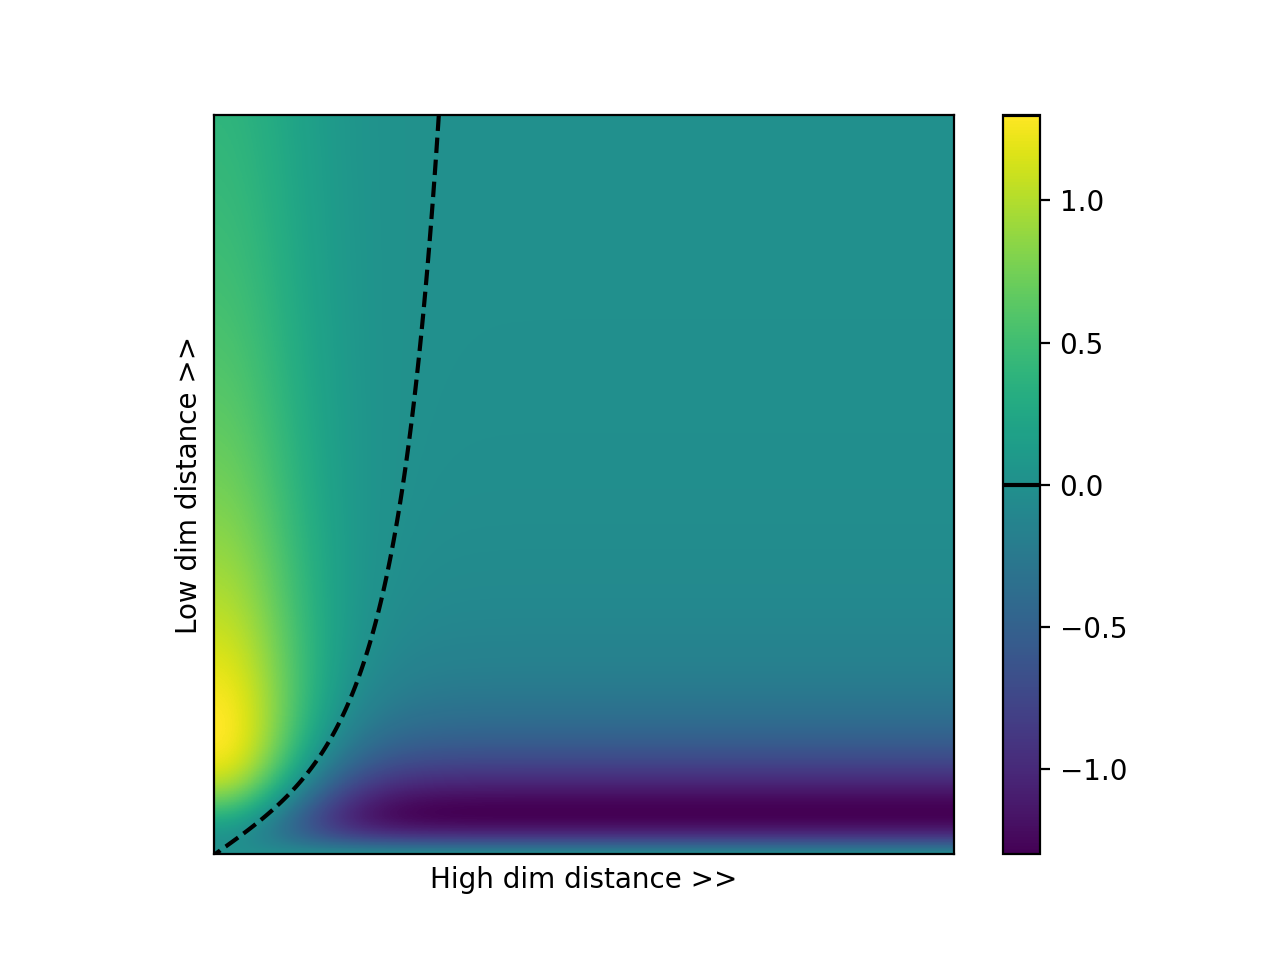
\includegraphics[width=7cm]{tex_images/tsne_grad.png} }}%
% 	\qquad
% 	\subfloat[\centering UMAP gradients]{{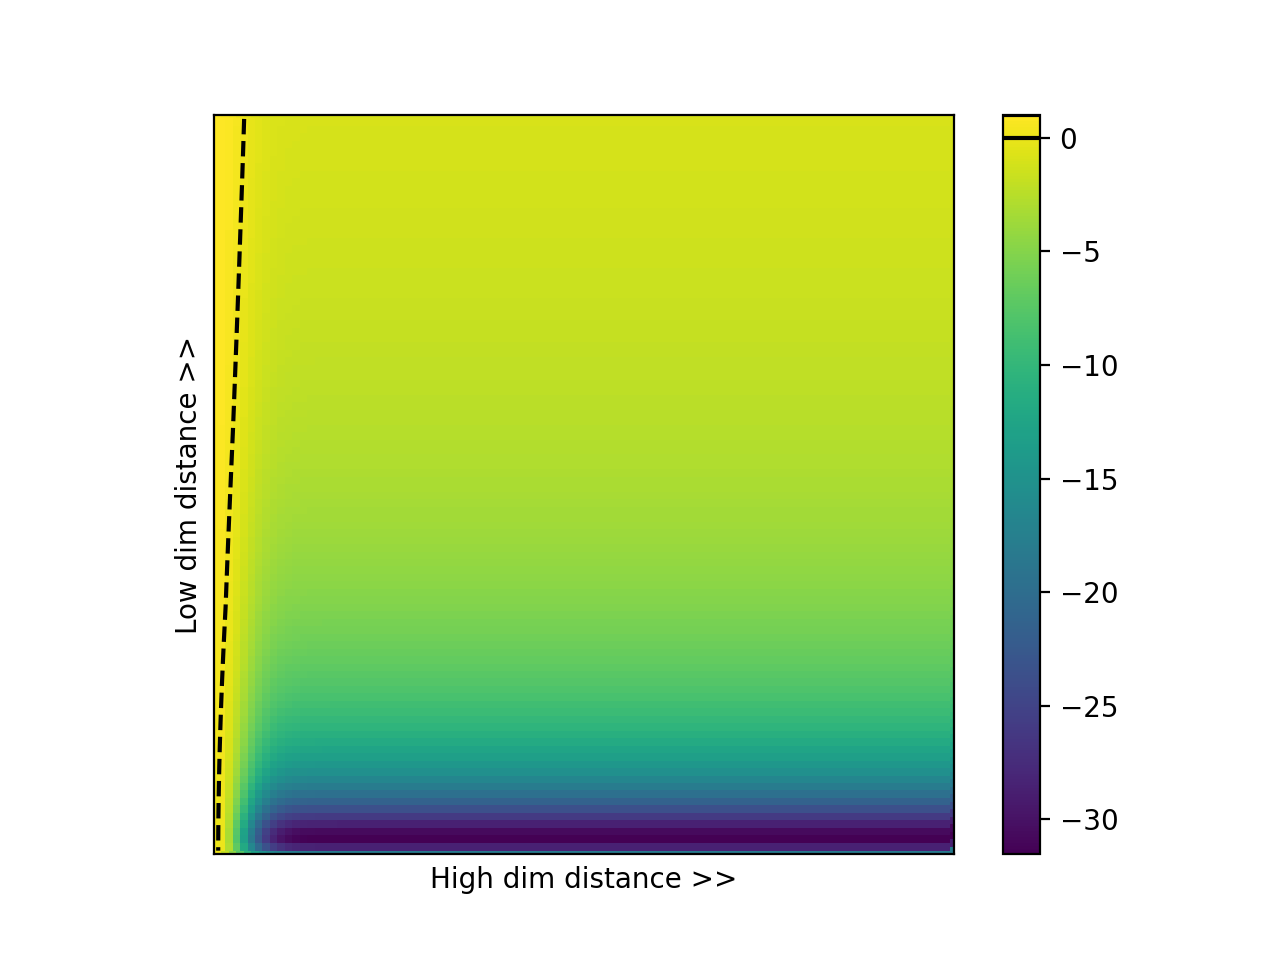
\includegraphics[width=7cm]{tex_images/umap_grad.png} }}%
% 	\caption{A comparison of tSNE and UMAP gradients for linearly growing distances}%
% 	\label{fig:linear_grads}%
% \end{figure}
% 
% \begin{figure}
% \centering
% 	\subfloat[\centering tSNE gradients]{{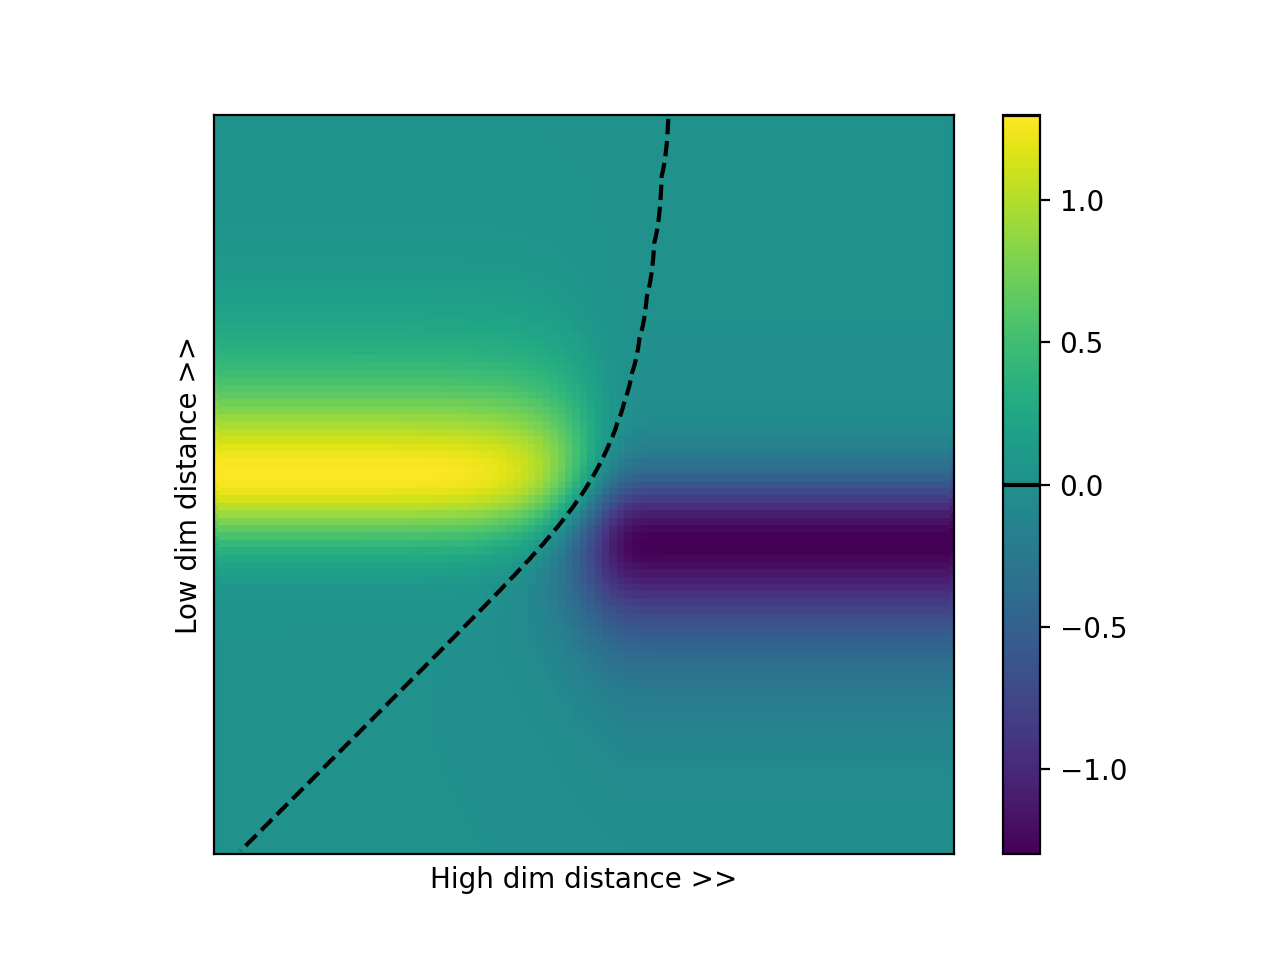
\includegraphics[width=7cm]{tex_images/tsne_exp_grads.png} }}%
% 	\qquad
% 	\subfloat[\centering UMAP gradients]{{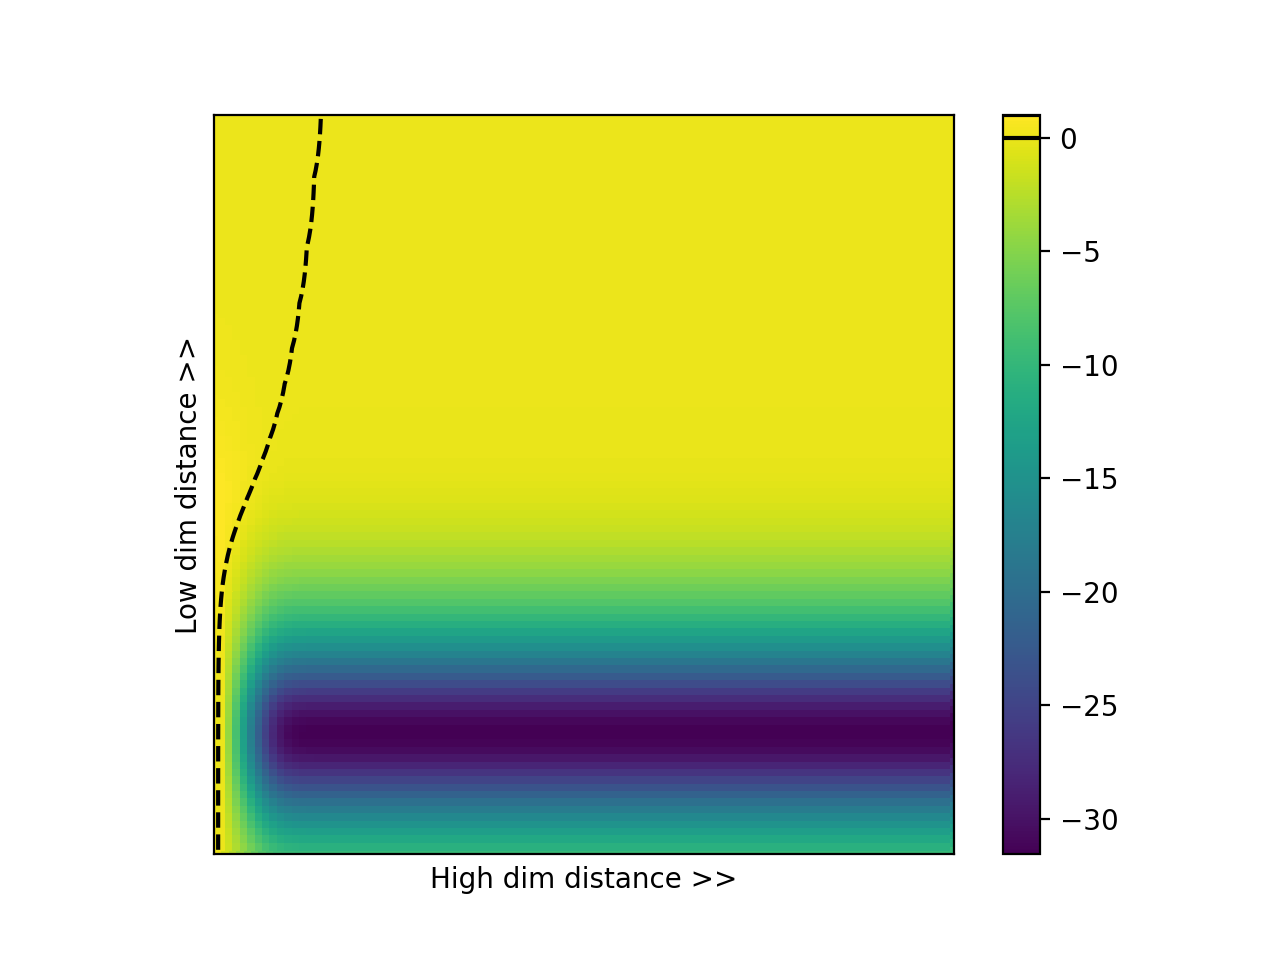
\includegraphics[width=7cm]{tex_images/umap_exp_grads.png} }}%
% 	\caption{A comparison of tSNE and UMAP gradients for exponentially growing distances}%
% 	\label{fig:exp_grads}%
% \end{figure}
% 
% \subsection{Implementation differences} \label{implementation_diffs}
% Given the above descriptions of the algorithms, we now describe specific implementation differences between the two. Section \ref{results} will discuss the
% practical effect that each of these has on the results.
% 
% \begin{itemize}
%     \item tSNE collects all of the attractive and repulsive forces before applying momentum gradient descent across every point simultaneously. In contrast,
%         UMAP updates the position of every point directly upon calculating its attractive and repulsive forces.
%     \begin{itemize}
%         \item Accordingly, UMAP applies attractive and repulsive forces iteratively by calculating $k$ random repulsive forces for every attractive force along the
%             nearest neighbor edges.
%         \item In contrast, tSNE similarly calculates attractions along each edge but estimates each point's repulsions across the entire dataset with Barnes-Hut
%             trees.
%     \end{itemize}
% 
%     \item tSNE's gradient descent has an additional scalar that amplifies the forces if a point moves in the same direction at time $t+1$ as it did at time $t$
%         and dampens the forces otherwise.
% 
%     \item UMAP finds approximate nearest neighbors using nearest-neighbor descent whereas tSNE takes the time to exactly identify nearest neighbor relationships.
% 
%     \item UMAP's high dimensional kernel on points $x_i$ and $x_j$ subtracts the minimum distance $\rho_i = \min_{k \neq i} d(x_i, x_k)$. The theoretical
%         justification for this is discussed at length in the UMAP paper. 
% 
%     \item tSNE symmetrizes the high-dimensional kernels with $S_{tsne}(p_{j|i}, p_{i|j}) = (p_{j|i} + p_{i|j}) / 2$ while UMAP uses a probabilistic
%         symmetrization with $S_{umap}(p_{j|i}, p_{i|j}) = p_{j|i} + p_{i|j} - p_{j|i} \cdot p_{i|j}$
% 
%     \item tSNE performs random initialization whereas UMAP initializes with a Laplacian eigenmap projection.
% 
%     \item UMAP applies the attractive force between $y_i$ and $y_j$ to both $y_i$'s and $y_j$'s positions whereas tSNE applies the attractive force to only $y_i$.
%         We refer to these options as \textit{symmetric} and \textit{asymmetric} attraction.
% \end{itemize}
% 
% \subsection{Uniform UMAP} \label{uniform}
% We must make a few modifications to either UMAP's or tSNE's optimization methodology in order to perform a fully controlled comparison between the two. The principle obstacle is that
% UMAP performs live gradient updates on each point (which precludes the use of momentum gradient descent) while tSNE collects the gradients across the entire
% dataset before applying them simultaneously. This complicates comparing the two as tSNE normalizes repulsive forces by the sum over all kernels $Z$,
% therefore making it impossible to implement tSNE within UMAP's original framework. Specifically, UMAP would require access to all the repulsions for
% normalization but applies the repulsions before all of them have been collected.
% 
% UMAP's original algorithm approximates the $p_{ij}$ and $(1 - p_{ij})$ scalars in the attractive and repulsive forces by selectively applying attractions
% and repulsions per epoch. Namely, the attractive and repulsive forces are applied on any given epoch with likelihood proportional to $p_{ij}$
% or $(1 - p_{ij})$. Thus if a force was applied on epoch $i$ it will not necessarily be performed on epoch $i+1$. Note that this choice was not necessitated by theoretical derivations
% and can be modified without sacrificing the theoretical soundness of the UMAP algorithm.
% 
% We would instead like to implement UMAP such that we uniformly calculate one repulsion for every attraction in order to neatly collect all of forces before
% normalizing and performing gradient descent. To do this, note that the nearest-neighbor edge weights $p_{ij}$ are available to us during
% optimization. In order to approximate the $(1 - p_{ij})$ scalars, however, we hypothesize that they will
% effectively average out when applied to random pairs of points over many repulsions. We therefore replace the sampling scheme by doing one repulsion for every attraction and scaling the repulsive force by $(1 - \bar{p}_{ij})$, where
% $\bar{p}_{ij}$ is the mean high-dimensional kernel value. We experimentally validate this decision in table ?? and show that this achieves identical results to UMAP across datasets and metrics.
% 
% We name this modified UMAP implementation \textit{Uniform UMAP} and note that it has several structural advantages to the original method. 
% \begin{itemize}
%         \item Uniform UMAP removes the need for calculating multiple repulsions during the sampling schema, cutting down on the number of force calculations by $n-1$, where $n$ is the number of repulsions performed when the repulsive forces are sampled.
%         \item We can now easily collect gradients across the entire dataset, allowing us to apply techniques like momentum gradient descent for quicker convergence.
%         \item The repulsions no longer depend on the epoch or edge weights, allowing us to effectively distribute force computations
%         \item When correctly modified to implement tSNE, Uniform UMAP removes tSNE's dependency on the computationally costly Barnes-Hut trees, obtaining a very
%             significant speedup over other tSNE implementations.
% \end{itemize}
% 
% With this change, we can use Uniform UMAP to obtain UMAP's results using full-dataset gradient descent as is done in tSNE.
% 
% % FIXME FIXME FIXME -- the below logic should work when normalized, since the repulsions aren't crazy strong
% % The second major modification has to do with the iterative nature of the gradient descent epochs. Consider the following common situation: assume during
% % epoch $t$ that we apply an attraction along the edge $(y_i, y_j)$ and then a repulsion along $(y_i, y_k)$. Then, in epoch $t+1$ we once again attract along
% % $(y_i, y_j)$ and repel along $(y_i, y_l)$. Due to randomness, many individual repulsive forces will negligibly affect the embedding. Thus the two attractive forces,
% % originally separated by a repulsion, can be approximated by performing the attraction $(y_i, y_j)$ at time $t$ twice, followed by applying the two repulsive
% % forces in tandem. Generalizing this logic, we note that applying a $k$-times stronger attractive force with $k$ random repulsions approximates the iterative
% % nature of UMAP and tSNE, with approximations worsening as $k$ grows.
% % Furthermore, if we intend to apply an attractive force $k$ times then we can calculate apriori how much the force will diminish with each application. Thus, we can be
% % more sophisticated than simply scaling the force linearly by the number of repeated applications. \textit{It remains to identify when this approximation is appropriate
% % and to what extent it is correct}.
% 
% \section{Embedding Results} \label{results}
% We now show that, subject to the change in \ref{uniform}, one can directly implement both tSNE and UMAP through either framework. We first show that Uniform UMAP
% can successfully recreate UMAP's outputs across a variety of datasets. Then, we go through the elements in \ref{implementation_diffs} to identify what effect
% each choice has on the tSNE and Uniform UMAP embeddings. Using this, we identify the changes necessary to produce tSNE's outputs within the UMAP framework and vice versa.
% 
% \subsection{Metrics}
% To avoid relying on qualitative observation, we introduce several metrics that we will be using to describe both embedding quality and the differences between tSNE and UMAP.
% 
% Want one metric that is ``quality of embedding'' and one that captures ``amount of space between clusters''. For the latter, it should be enough to get
% distances of all points between two clusters and take the 1\% cut. Basically, something to give you the distance between the shells of the two clusters.
% % \begin{enumerate}
% %     \item Change in sort index - If we sort the high-dimensional distances and the low-dimensional distances, how different are the sort indices? The x-axis
% %         goes through all the high-dimensional distances in order; the y-axis is the relative change for that high-dimensional sort index
% %     \item High dimensional distance vs. low dimensional distance - These are simply the low-dimensional distances plotted vs. the high dimensional distances. The high dimensional distances
% %         have been sorted from least to greatest. Note that PCA is a straight line (which is what we expected). Also, note that the large high-dim distances are
% %         represented by larger low-dim distances in UMAP than in tSNE
% %     \item Sorted distances - This is just the y-values of the previous plot. Basically, when we sort the high-dimensional distances, what do the low
% %         dimensional ones look like?
% %     \item Nearest neighbor overlap - For every point, what percent of its [k, k + 10] nearest neighbors are preserved? Note that immediate local distances are preserved in
% %         tSNE and UMAP, after which there is a giant portion where the middle distances aren't relevant.
% %     \item Relative error - This is the relative error for high-dimensional distances. We normalize both the high-dim and low-dim distances to $[0, 1]$, since the
% %         magnitudes are arbitrary in our setting. Thus, we do $| (d^h(x_i, x_j) - d^l(y_i - y_j)) |/ d^h(x_i, x_j)$. We replace the 0's in the high dimensional
% %         distances with 1's to avoid division errors.
% % \end{enumerate}
% 
% \subsection{UMAP and Uniform UMAP Equivalency}
% 
% \subsection{Analysis of Implementation Choices}
% 
% \subsection{Achieving tSNE within UMAP}
% The main obstacle to overcome is undoing the normalization
% differences between tSNE and UMAP. In fact, tSNE can be achieved within the UMAP implementation through the following modifications:
% \begin{enumerate}
%     \item Normalize the high- and low-dimensional kernels as they are normalized in tSNE
%     \item Perform tSNE's gradient descent as described in \ref{uniform}
%     \item Apply asymmetric attraction forces
% \end{enumerate}
% Due to using tSNE's normalization, we also require the corresponding modification to the KL divergence. As such, we obtain gradients
% \begin{align*}
%     F_{attr} &= 4 \sum_{j \neq i} p_{ij} q_{ij} Z (y_i - y_j) \\
%    F_{rep} &= 4 \sum_{j \neq i} q_{ij}^2 Z (y_i - y_j)
% \end{align*}
%    where
% \begin{align*}
%    q_{ij} &= \dfrac{(1 + a ||y_i - y_j||_2^{2b})^{-1}}{\sum_{k \neq l} (1 + a ||y_i - y_j||_2^{2b})^{-1}} \\
%     p_{j|i} &= \dfrac{\text{exp}( -(d(x_i, x_j)^2 - \rho_i) / \tau_i)}{\sum_{k \neq l} \text{exp}( (-d(x_k, x_l)^2 + \rho_i) / \tau_k)}
% \end{align*}
%    and $Z = \sum_{k \neq l} (1 + a ||y_i
%    - y_j||_2^{2b})^{-1}$. Notice that this is essentially the tSNE kernels with UMAP's $\rho_i$, $a$, and $b$ scalars. We show later that these can be removed
%    in practice.
% 
% \subsection{Achieving UMAP within tSNE}
% This direction turns out to be significantly easier. Performing the Barnes-Hut algorithm for tSNE with a Laplacian eigenmap initialization and symmetric
% attraction is sufficient to obtain UMAP consistently.
% 
% \subsection{Claims and misconceptions}
% % FIXME - talk about GAINS in tSNE optimization
% We would like to discuss several claims regarding these algorithms' choices and use-cases. Firstly, we'd like to note that the tSNE paper mentions
% that the high-dimensional probabilities $p_{j|i}$ are normalized by the sum $\sum_{k \neq i} \exp\left( ||y_i - y_k||^2 \right) / \tau_i$. To the authors of
% this paper and other people whom we've spoken to, this implies that the normalization occurs across rows of the pairwise probability matrix. Instead, tSNE
% implementations normalize $p_{j|i}$ across the entire pairwise probability matrix, giving us symmetric normalizations in the high- and low-dimensional spaces (a
% necessary condition for the KL divergence).
% 
% Additionally, there are several choices made in UMAP that do not provide practical changes. Namely, we find that the choice of normalization is the
% single necessary condition for switching between tSNE and UMAP.
% This puts the practical necessity of multiple components of UMAP's algorithm into question. The first of these is the pseudo-distance metric $\tilde{d}_i(x_j, x_k) = ||x_j - x_k||_2^2
% - \rho_i$. Its inclusion theoretically justifies that the nearest-neighbor graph captures the topology of the high-dimensional dataset. Despite the sound
% theoretical derivations we find across datasets, metrics, and contexts that subtracting the minimum distance has a negligible effect on the resulting
% embeddings. We also refute the assertion that tSNE's lack of a mathematical framework prohibits it from being
% extended; specific examples include embedding unseen
% points given an existing projection, utilizing categorical variables, and consolidating differing metrics. Our implementation of Uniform UMAP is able
% to, under tSNE's normalization and optimization schema, perform all of these tasks in the same manner as UMAP while obtaining results in line with tSNE's. Lastly, there have been claims made that tSNE
% with the Laplacian eigenmap initialization recreates UMAP's outputs \cite{kobak2019umap} or that the initialization is primarily responsible for the quality of
% the resulting embedding \cite{kobak2021initialization}. While this may be true for certain datasets, we do not observe it to be the case universally.


\bibliographystyle{ACM-Reference-Format}
\bibliography{references}

\end{document}
\endinput
